%!TEX encoding = UTF-8 Unicode
%!TEX root = ../exercises.tex

\ifPreSolution
\Exercise{\ExeWeekONE}\label{exe:W01}

\begin{Goals}
%!TEX encoding = UTF-8 Unicode

\item Förstå vad som händer när satser exekveras och uttryck evalueras.
\item Förstå sekvens, alternativ och repetition.
\item Känna till literalerna för enkla värden, deras typer och omfång.
\item Kunna deklarera och använda variabler och tilldelning, samt kunna rita bilder av minnessituationen då variablers värden förändras.
\item Förstå skillnaden mellan olika numeriska typer, kunna omvandla mellan dessa och vara medveten om noggrannhetsproblem som kan uppstå.
\item Förstå booleska uttryck och värdena \code{true} och \code{false}, samt kunna förenkla booleska uttryck.
\item Förstå skillnaden mellan heltalsdivision och flyttalsdivision, samt användning av rest vid heltalsdivision.
\item Förstå precedensregler och användning av parenteser i uttryck.
\item Kunna använda \code{if}-satser och \code{if}-uttryck.
\item Kunna använda \code{for}-satser och \code{while}-satser.
\item Kunna använda \code{math.random()} för att generera slumptal i olika intervaller.
\item Kunna beskriva skillnader och likheter mellan en procedur och en funktion.

\end{Goals}

\begin{Preparations}
\item \StudyTheory{01}
\item Du behöver en dator med Scala och Kojo installerad, se appendix~\ref{appendix:compile} och  \ref{appendix:kojo}.
\end{Preparations}

\else

\ExerciseSolution{\ExeWeekONE}

\fi  %%% END \ifPreSolution


\BasicTasks
%%%% TODO Strukturera övningen annorlunda: atomer, sammansatta uttryck, funktiner, kojo ??}


\def\what{\emph{Para ihop begrepp med beskrivning.}}

\QUESTBEGIN

\Task \what

\vspace{1em}\noindent Koppla varje begrepp med den (förenklade) beskrivning som passar bäst: 

\begin{ConceptConnections}
  litteral & 1 & & A & kan inträffa medan programmet kör \\ 
  sträng & 2 & & B & att översätta kod till exekverbar form \\ 
  sats & 3 & & C & vid anrop beräknas ett returvärde \\ 
  uttryck & 4 & & D & decimaltal med begränsad noggrannhet \\ 
  funktion & 5 & & E & bra då antalet repetitioner är bestämt i förväg \\ 
  procedur & 6 & & F & en kodrad som gör något; kan särskiljas med semikolon \\ 
  exekveringsfel & 7 & & G & beskriver vad data kan användas till \\ 
  kompileringsfel & 8 & & H & antingen sann eller falsk \\ 
  abstrahera & 9 & & I & för att ändra en variabels värde \\ 
  kompilera & 10 & & J & kombinerar värden och funktioner till ett nytt värde \\ 
  typ & 11 & & K & en sekvens av tecken \\ 
  for-sats & 12 & & L & att införa nya begrepp som förenklar kodningen \\ 
  while-sats & 13 & & M & anger ett specifikt datavärde \\ 
  tilldelning & 14 & & N & kan inträffa innan exekveringen startat \\ 
  flyttal & 15 & & O & bra då antalet repetitioner ej är bestämt i förväg \\ 
  boolesk & 16 & & P & vid anrop sker (sido)effekt; returvärdet är tomt \\ 
\end{ConceptConnections}

\SOLUTION

\TaskSolved \what

\begin{ConceptConnections}
  litteral & 1 & ~~\Large$\leadsto$~~ &  D & anger ett specifikt datavärde \\ 
  sträng & 2 & ~~\Large$\leadsto$~~ &  G & en sekvens av tecken \\ 
  sats & 3 & ~~\Large$\leadsto$~~ &  F & en kodrad som gör något; kan särskiljas med semikolon \\ 
  uttryck & 4 & ~~\Large$\leadsto$~~ &  H & kombinerar värden och funktioner till ett nytt värde \\ 
  funktion & 5 & ~~\Large$\leadsto$~~ &  K & vid anrop beräknas ett returvärde \\ 
  procedur & 6 & ~~\Large$\leadsto$~~ &  J & vid anrop sker (sido)effekt; returvärdet är tomt \\ 
  exekveringsfel & 7 & ~~\Large$\leadsto$~~ &  N & kan inträffa medan programmet kör \\ 
  kompileringsfel & 8 & ~~\Large$\leadsto$~~ &  M & kan inträffa innan exekveringen startat \\ 
  abstrahera & 9 & ~~\Large$\leadsto$~~ &  A & att införa nya begrepp som förenklar kodningen \\ 
  kompilera & 10 & ~~\Large$\leadsto$~~ &  C & att översätta kod till exekverbar form \\ 
  typ & 11 & ~~\Large$\leadsto$~~ &  I & beskriver vad data kan användas till \\ 
  for-sats & 12 & ~~\Large$\leadsto$~~ &  O & bra då antalet repetitioner är bestämt i förväg \\ 
  while-sats & 13 & ~~\Large$\leadsto$~~ &  P & bra då antalet repetitioner ej är bestämt i förväg \\ 
  tilldelning & 14 & ~~\Large$\leadsto$~~ &  L & för att ändra en variabels värde \\ 
  flyttal & 15 & ~~\Large$\leadsto$~~ &  E & decimaltal med begränsad noggrannhet \\ 
  boolesk & 16 & ~~\Large$\leadsto$~~ &  B & antingen sann eller falsk \\ 
\end{ConceptConnections}

\QUESTEND






\def\what{\emph{Utskrift i Scala REPL.}}

\QUESTBEGIN

\Task \what 

\vspace{1em}\noindent Starta Scala REPL \Eng{Read-Evaluate-Print-Loop}.

\begin{REPLnonum}
$ scala
Welcome to Scala version 2.11.8 (Java HotSpot(TM) 64-Bit Server VM, Java 1.8).
Type in expressions to have them evaluated.
Type :help for more information.

scala> 
\end{REPLnonum}

\Subtask Skriv efter prompten \code{scala>} en sats som skriver ut en valfri (bruklig/knasig) hälsningsfras, genom anrop av proceduren \code{println} med något strängargument. Tryck på \textit{Enter} så att satsen kompileras och exekveras. 

\Subtask Skriv samma sats igen (eller tryck pil-upp) men ''glöm bort'' att skriva högerparentesen efter argumentet innan du trycker på \textit{Enter}. Vad händer?

\begin{framed}
\noindent\emph{Tips inför fortsättningen:} Det finns många användbara kortkommandon och andra trix för att jobba snabbt i REPL. Be gärna någon som kan dessa trix att visa dig hur man kan jobba snabbare. Läs appendix \ref{appendix:compile:REPL} och prova sedan att kopiera och klistra in text. Använd piltangenterna för att bläddra i historiken och Ctrl+A för att komma till början av raden, Ctrl+K för att radera resten av raden, etc.
\end{framed}



\SOLUTION 
\TaskSolved \what

\SubtaskSolved Till exempel:
\begin{REPLnonum}
scala> println("hejsan svejsan")
\end{REPLnonum}

\SubtaskSolved Om högerparentes fattas får man fortsätta skriva på nästa rad. Detta indikeras med vertikalstreck i början av varje ny rad:
\begin{REPLnonum}
scala> println("hejsan svejsan"
     | + "!" 
     | )
hejsan svejsan!
\end{REPLnonum}

\QUESTEND



\def\what{\emph{Konkatenering av strängar.}}

\QUESTBEGIN

\Task \what

\Subtask Skriv ett uttryck som konkatenerar två strängar, t.ex. \code{"gurk"} och \code{"burk"}, med hjälp av operatorn \code{+} och studera resultatet. Vad har uttrycket för värde och typ? Vilken siffra står efter ordet \code{res} i variabeln som lagrar resultatet?

\Subtask Använd resultatet från konkateneringen, t.ex. \code{res0} (byt ev. ut \code{0}:an mot siffran efter \code{res} i utskriften från förra evalueringen), och skriv ett uttryck med hjälp av operatorn \code{*} som upprepar resultatet från förra deluppgiften 42 gånger. 


\SOLUTION

\TaskSolved \what

\SubtaskSolved 
\begin{REPLnonum}
scala> "gurk" + "burk"
res1: String = gurkburk
\end{REPLnonum}
värde: \code{"gurkburk"}, typ:  \code{String}

\SubtaskSolved
\begin{REPLnonum}
scala> res1 * 42
res2: String = gurkatomatgurkatomatgurkatomatgurkatomatgurkatomatgurkatomatgurkatomatgurkatomatgurkatomatgurkatomatgurkatomatgurkatomatgurkatomatgurkatomatgurkatomatgurkatomatgurkatomatgurkatomatgurkatomatgurkatomatgurkatomatgurkatomatgurkatomatgurkatomatgurkatomatgurkatomatgurkatomatgurkatomatgurkatomatgurkatomatgurkatomatgurkatomatgurkatomatgurkatomatgurkatomatgurkatomatgurkatomatgurkatomatgurkatomatgurkatomatgurkatomatgurkatomat
\end{REPLnonum}

\QUESTEND




\def\what{\emph{När upptäcks felet?}}

\QUESTBEGIN

\Task \what 

\Subtask Vad har uttrycket \code{ "hej" * 3 } för typ och värde? Testa i REPL.

\Subtask Byt ut 3:an ovan mot ett så pass stort heltal så att minnet blir fullt. Hur börjar felmeddelandet? Är detta ett körtidsfel eller ett kompileringsfel?

\Subtask Välj ett värde på argumentet efter operatorn \code{*} så att ett typfel genereras. Hur börjar felmeddelandet? Är detta ett körtidsfel eller ett kompileringsfel?

\begin{framed}
\noindent\emph{Tips inför fortsättningen:} Gör gärna fel när du kodar så lär du dig mer! Träna på att tolka olika felmeddelanden och fråga någon om hjälp om du inte förstår. Kompilatorns utskrifter kan vara till stor hjälp, men är ibland kryptiska. Om du kör fast och inte kommer vidare själv så be om hjälp, \emph{men be om tips snarare än färdiga lösningar} så att du behåller initiativet själv och tar kontroll över nästa steg i ditt lärande.
\end{framed}


\SOLUTION

\TaskSolved \what

\SubtaskSolved Typ: \code{String}, värde: \code{"hejhejhej"}

\SubtaskSolved Körtiddsfel:
\begin{REPLnonum}
scala> "hej" * Int.MaxValue
java.lang.OutOfMemoryError: Java heap space
\end{REPLnonum}

\SubtaskSolved Kompileringsfel: (indikeras av texten \code{<console> ... error:})
\begin{REPLnonum}
scala> "hej" * true
<console>:12: error: type mismatch;
 found   : Boolean(true)
 required: Int
       "hej" * true
\end{REPLnonum}


\QUESTEND




\def\what{\emph{Litteraler och typer.}}

\QUESTBEGIN

\Task \what

\Subtask Ta hjälp av REPL-kommadot \verb+:type+ (kan förkortas \code{:t}) vid behov för att para ihop nedan litteraler med rätt typ. 

\begin{ConceptConnections}[0.35\textwidth]
  \code|1    | & 1 & & A & \code|Float  | \\ 
  \code|1L   | & 2 & & B & \code|Double | \\ 
  \code|1.0  | & 3 & & C & \code|Unit   | \\ 
  \code|1D   | & 4 & & D & \code|Int    | \\ 
  \code|1F   | & 5 & & E & \code|Boolean| \\ 
  \code|'1'  | & 6 & & F & \code|Long   | \\ 
  \code|"1"| & 7 & & G & \code|String | \\ 
  \code|true | & 8 & & H & \code|Double | \\ 
  \code|false| & 9 & & I & \code|Char   | \\ 
  \code|()   | & 10 & & J & \code|Boolean| \\ 
%\Connect{\code|1      |}  {\code|Int    |}
%\Connect{\code|1L     |}  {\code|Long   |}
%\Connect{\code|1.0    |}  {\code|Double |}
%\Connect{\code|1D     |}  {\code|Double |}
%\Connect{\code|1F     |}  {\code|Float  |}
%\Connect{\code|'1'    |}  {\code|Char   |}
%\Connect{\code|\"1\"  |}  {\code|String |}
%\Connect{\code|true   |}  {\code|Boolean|} 
%\Connect{\code|false  |}  {\code|Boolean|} 
%\Connect{\code|()     |}  {\code|Unit   |} 
\end{ConceptConnections}

\Subtask Vad händer om du adderar 1 till det största möjliga värdet av typen \code{Int}? 
\\\emph{Tips:} se snabbreferensen \footnote{\url{http://cs.lth.se/pgk/quickref/}} under rubriken ''The Scala type system'' avsnitt ''Methods on numbers''.

\Subtask Vad är skillnaden mellan typerna \code{Long} och \code{Int}?

\Subtask Vad är skillnaden mellan typerna \code{Double} och \code{Float}?


\SOLUTION

\TaskSolved \what

\SubtaskSolved 

\begin{ConceptConnections}
  \code|1    | & 1 & ~~\Large$\leadsto$~~ &  C & \code|Int    | \\ 
  \code|1L   | & 2 & ~~\Large$\leadsto$~~ &  F & \code|Long   | \\ 
  \code|1.0  | & 3 & ~~\Large$\leadsto$~~ &  J & \code|Double | \\ 
  \code|1D   | & 4 & ~~\Large$\leadsto$~~ &  D & \code|Double | \\ 
  \code|1F   | & 5 & ~~\Large$\leadsto$~~ &  B & \code|Float  | \\ 
  \code|'1'  | & 6 & ~~\Large$\leadsto$~~ &  A & \code|Char   | \\ 
  \code|"1"| & 7 & ~~\Large$\leadsto$~~ &  E & \code|String | \\ 
  \code|true | & 8 & ~~\Large$\leadsto$~~ &  G & \code|Boolean| \\ 
  \code|false| & 9 & ~~\Large$\leadsto$~~ &  I & \code|Boolean| \\ 
  \code|()   | & 10 & ~~\Large$\leadsto$~~ &  H & \code|Unit   | \\ 
%\ConnectSolved{\code|1      |}  {\code|Int    |}
%\ConnectSolved{\code|1L     |}  {\code|Long   |}
%\ConnectSolved{\code|1.0    |}  {\code|Double |}
%\ConnectSolved{\code|1D     |}  {\code|Double |}
%\ConnectSolved{\code|1F     |}  {\code|Float  |}
%\ConnectSolved{\code|'1'    |}  {\code|Char   |}
%\ConnectSolved{\code|\"1\"  |}  {\code|String |}
%\ConnectSolved{\code|true   |}  {\code|Boolean|} 
%\ConnectSolved{\code|false  |}  {\code|Boolean|} 
\end{ConceptConnections}

\SubtaskSolved Värdet går över gränsen för vad som får plats i ett 32 bitars heltal och ''börjar om'' på det minsta möjliga heltalet \code{Int.MinValue}
\begin{REPL}
scala> Int.MaxValue + 1
res3: Int = -2147483648

scala> Int.MinValue
res4: Int = -2147483648
\end{REPL}

\SubtaskSolved Båda är heltal men \code{Long} kan representera större tal än \code{Int}.

\SubtaskSolved Båda är flyttal men \code{Double} har dubbel precision och kan representera större tal med fler decimaler.



\QUESTEND





\def\what{\emph{Matematiska funktioner. Scaladoc.}}

\QUESTBEGIN

\Task \what

\Subtask Antag att du har ett schackbräde med 64 rutor. Tänk dig att du börjar med ett enda riskorn på första rutan och sedan lägger dubbelt så många riskorn i en ny hög för varje efterföljande ruta: 1, 2, 4, 8, ...  etc. Hur många riskorn\footnote{\url{https://en.wikipedia.org/wiki/Wheat_and_chessboard_problem}} blir det då i den sextiofjärde rishögen?

\emph{Tips:} Du ska beräkna $2^{64} - 1$. Om du skriver \code{math.} i REPL och trycker TAB får du se inbyggda matematiska funktioner i Scalas standardbibliotek:
\begin{REPL}
scala> math.    // Tryck TAB direkt efter punkten och betrakta listan
\end{REPL}
Använd funktionen \code{math.pow} och lämpliga argument. Om du skriver \code{math.pow} och trycker TAB \emph{två gånger} får du se funktionshuvudet med parameterlistan. 

Om du surfar till \url{http://www.scala-lang.org/api/current/} och skriver \code{math} i sökrutan och sedan, efter att du klickat på \textbf{\textsf{\small scala.math}}, skriver \textbf{\textsf{\small pow}} i rutan längre ner, så filtreras sidan och du hittar dokumentationen av \code{ def pow } som du kan klicka på och läsa mer om.   

\Subtask Definiera funktionen \code{omkrets} nedan i REPL. Går det bra att utelämna returtyp-annoteringen? Varför? Finns det anledning att ha den kvar?
\begin{Code}
def omkrets(radie: Double): Double = 2 * math.Pi * radie
\end{Code}

\Subtask Jordens (genomsnittliga) diameter (vid ekvatorn) är ca $12 750$ $km$. Anropa funktionen \code{omkrets} ovan för att beräkna hur många kilometer per dag man ungefär måste färdas om man vill åka jorden runt på 80 dagar. 

\SOLUTION

\TaskSolved \what

\SubtaskSolved Ja, returtyp-annoteringen \code{: Double} kan utelämnas. 

\begin{itemize}
\item Varför kan returtyp utelämnas?\\Eftersom kompilatorns typhärledning kan härleda returtypen. 
\item Varför kan man vilja utelämna den?\\Det blir kortare att skriva utan. 
\item Anledningar att ange returtyp: 
\begin{itemize}
\item  Med explicit returtyp får du hjälp av kompilatorn att redan under kompileringen kontrollera att uttrycket till höger om likhetstecknet har den typ som förväntas. 

\item Genom att du anger returtypen explicit får de som enbart läser metodhuvudet (och inte implementationen)
 tydligt se vad som returneras.
\end{itemize}
\end{itemize}	


\SubtaskSolved Beräkning av $2^{64} - 1$ med \code{math.pow} enligt nedan ger ungefär $1.8 \cdot 10^{19}$
\begin{REPL}
scala> math.pow(2, 64) - 1
res0: Double = 1.8446744073709552E19
\end{REPL}


\SubtaskSolved Ca $500$ $km$.
\begin{REPL}
scala> omkrets(12750 / 2) / 80
res0: Double = 500.6913291658733
\end{REPL}

\QUESTEND




\def\what{\emph{Förändringsbara variabler och tilldelning.}}

\QUESTBEGIN

\Task \what~Rita en \emph{ny} bild av datorns minne efter \emph{varje} exekverad rad 1--6 nedan. Varje bild ska visa alla variabler som finns i minnet och deras variabelnamn, typ och värde.

\begin{REPL}[numbers=left, numberstyle=\color{black}\ttfamily\scriptsize\selectfont]
scala> var a = 13
scala> var b = a + 1
scala> var c = (a + b) * 2.0
scala> b = 0
scala> a = 0
scala> c = c + 1
\end{REPL}
Efter första raden ser minnessituationen ut så här:

\MEM{a}{Int}{13}

\SOLUTION

\TaskSolved \what

\begin{tabular}{l l l}
\MEM{{\it Efter rad1:~~~~} a}{Int}{13}\\
\MEM{{\it Efter rad2:~~~~} a}{Int}{13} & \MEM{b}{Int}{14}\\
\MEM{{\it Efter rad3:~~~~} a}{Int}{13} & \MEM{b}{Int}{14} & \MEM{c}{Double}{54.0}\\
\MEM{{\it Efter rad4:~~~~} a}{Int}{13} & \MEM{b}{Int}{0} & \MEM{c}{Double}{54.0}\\
\MEM{{\it Efter rad5:~~~~} a}{Int}{0} & \MEM{b}{Int}{0} & \MEM{c}{Double}{54.0}\\
\MEM{{\it Efter rad6:~~~~} a}{Int}{0} & \MEM{b}{Int}{0} & \MEM{c}{Double}{55.0}\\
\end{tabular}

\QUESTEND


\def\what{\emph{Slumptal med \code{math.random}.}}

\QUESTBEGIN

\Task\label{exercise:expressions:roll} \what

\Subtask Vad ger funktionen \code{math.random} för resultatvärde? Vilken typ? Vad är största och minsta möjliga värde?
\\\emph{Tips:} Se scaladoc här: \Scaladoc och prova i REPL.

\Subtask Deklarera den parameterlösa funktionen \code{def roll: Int = ???} som ska representera ett tärningskast och ge ett slumpmässigt heltal mellan 1 och 6. Testa funktionen genom att anropa den många gånger. \\\emph{Tips:} Använd \code{math.random} och multiplicera och addera med lämpliga heltal. Omge beräkningen med parenteser och avsluta med \code{.toInt} för att avkorta decimaler och omvandla typen från \code{Double} till \code{Int}.

\SOLUTION

\TaskSolved \what

\SubtaskSolved Ur dokumentationen:
\begin{Code}
/** Returns a Double value with a positive sign, 
 *  greater than or equal to 0.0 and less than 1.0.
 */
def random(): Double
\end{Code}


\SubtaskSolved 
\begin{REPL}
scala> def roll: Int = (math.random * 6 + 1).toInt

scala> roll
res0: Int = 4

scala> roll
res1: Int = 1
\end{REPL}

\QUESTEND




\def\what{\emph{Repetition med \code{for}, \code{foreach} och \code{while}.}}

\QUESTBEGIN

\Task \what

\Subtask Så här kan en \code{for}-sats ser ut: 
\begin{Code}
for (i <- 1 to 10) print(i + ", ")
\end{Code}
Använd en \code{for}-sats för att skriva ut resultatet av 100 tärningskast med funktionen \code{roll} från uppgift \ref{exercise:expressions:roll}. 

\Subtask Så här kan en \code{foreach}-sats ser ut: 
\begin{Code}
(1 to 10).foreach { i => print(i + ",") }
\end{Code}
Använd en \code{foreach}-sats för att skriva ut resultatet av 100 tärningskast med funktionen \code{roll} från uppgift \ref{exercise:expressions:roll}. 

\Subtask Så här kan en \code{while}-sats ser ut: 
\begin{Code}
var i = 1
while (i <= 10) { print(i + ","); i = i + 1 }
\end{Code}
Använd en \code{while}-sats för att skriva ut resultatet av 100 tärningskast med funktionen \code{roll} från uppgift \ref{exercise:expressions:roll}. Vad händer om du glömmer \code{i = i + 1} ?


\SOLUTION

\TaskSolved \what

\SubtaskSolved \TODO

\QUESTEND


\def\what{\emph{Alternativ med \code{if}-sats och \code{if}-uttryck.}}

\QUESTBEGIN

\Task \what

\Subtask Så här kan en \code{if}-sats se ut (notera dubbla likhetstecken):
\begin{Code}
if (roll == 3) println("TRE") else println("INTE TRE") 
\end{Code}
Testa ovan i REPL. Skriv sedan en \code{for}-sats som kastar 100 tärningar och skriver ut strängen \code{"GRATTIS!"} om det blir en sexa, annars en ledsen smiley: \code{":("} 

\Subtask Så här kan ett \code{if}-uttryck se ut:
\begin{Code}
if (roll < 6) 0 else 1 
\end{Code}
Testa ovan i REPL. Skriv sedan en \code{while}-sats som kastar 100 tärningar och räknar antalet sexor. 

\SOLUTION

\TaskSolved \what

\SubtaskSolved \TODO

\QUESTEND



\def\what{\emph{Sekvens, sats och procedur.}}

\QUESTBEGIN

\Task \what

\Subtask Vad gör dessa satser? 
\begin{REPLnonum}
scala> def p = { print("san"); print("!"); println("hej")}
scala> p;p;p;p
\end{REPLnonum}

\Subtask
Använd pil-upp för att få tillbaka raden du skrev med definitionen av proceduren \code{p}. Byt plats på strängarna i utskriftsanropen i proceduren \code{p} så att utskriften blir: 
\begin{REPLnonum}
hejsan!
hejsan!
hejsan!
hejsan!
\end{REPLnonum}

\Subtask Hur tolkar kompilatorn klammerparenteser och semikolon?

\SOLUTION

\TaskSolved \what

\SubtaskSolved 
Satserna skapar denna utskrift:
\begin{REPLnonum}
san!hej
san!hej
san!hej
san!hej
\end{REPLnonum}

\SubtaskSolved 
\begin{REPLnonum}
scala> def p = { print("hej"); print("san"); println("!")}
scala> p;p;p;p
\end{REPLnonum}

\SubtaskSolved 
\begin{itemize}
\item Klammerparenteser används för att gruppera flera satser. Klammerparenteser behövs om man vill definiera en funktion som består av mer än en sats.  

\item Semikolon särskiljer flera satser. Semikolon behövs om man vill skriva många satser på samma rad.


\end{itemize}

\QUESTEND




\def\what{\emph{Heltalsdivision.}}

\QUESTBEGIN

\Task \what~Vilket värde och vilken typ hör till vilket uttryck?  Är du osäker på svaret, testa i REPL.

\begin{ConceptConnections}[0.3\textwidth]
  \code| 4 / 42      | & 1 & & A & \code|    4: Int      | \\ 
  \code| 42.0 / 2    | & 2 & & B & \code|   10: Int      | \\ 
  \code| 42 / 4      | & 3 & & C & \code| 21.0: Double   | \\ 
  \code| 42 % 4      | & 4 & & D & \code|true : Boolean  | \\ 
  \code| 4 % 42      | & 5 & & E & \code|false: Boolean  | \\ 
  \code| 40 % 4 == 0 | & 6 & & F & \code|    0: Int      | \\ 
  \code| 42 % 4 == 0 | & 7 & & G & \code|    2: Int      | \\ 
\end{ConceptConnections}

\SOLUTION

\TaskSolved \what

\begin{ConceptConnections}[0.3\textwidth]
  \code| 4 / 42      | & 1 & ~~\Large$\leadsto$~~ &  D & \code|    0: Int      | \\ 
  \code| 42.0 / 2    | & 2 & ~~\Large$\leadsto$~~ &  A & \code| 10.5: Double   | \\ 
  \code| 42 / 4      | & 3 & ~~\Large$\leadsto$~~ &  C & \code|   10: Int      | \\ 
  \code| 42 % 4      | & 4 & ~~\Large$\leadsto$~~ &  E & \code|    2: Int      | \\ 
  \code| 4 % 42      | & 5 & ~~\Large$\leadsto$~~ &  B & \code|    4: Int      | \\ 
  \code| 40 % 4 == 0 | & 6 & ~~\Large$\leadsto$~~ &  G & \code|true : Boolean  | \\ 
  \code| 42 % 4 == 0 | & 7 & ~~\Large$\leadsto$~~ &  F & \code|false: Boolean  | \\ 
\end{ConceptConnections}

\QUESTEND





\def\what{\emph{Booleska värden.}}

\QUESTBEGIN

\Task \what~Vilket värde har dessa uttryck?  % Uppgift 13

\Subtask \code{true && true}

\Subtask \code{false && true}

\Subtask \code{true || true}

\Subtask \code{false || true}

\Subtask \code{false || false}

\Subtask \code{true == true}

\Subtask \code{true != false}

\Subtask \code{true > false}

\Subtask \code{true && (1 / 0 > 1)}

\Subtask \code{false && (1 / 0 > 1)}

\SOLUTION

\TaskSolved \what

\SubtaskSolved \code{true}

\SubtaskSolved \code{false}

\SubtaskSolved \code{false}

\SubtaskSolved \code{true}

\SubtaskSolved \code{true}

\SubtaskSolved \code{false}

\SubtaskSolved \code{true}

\SubtaskSolved \code{true}

\SubtaskSolved Undantag kastas: \code{java.lang.ArithmeticException: / by zero}

\SubtaskSolved \code{false}

\QUESTEND





\def\what{\emph{Booleska variabler.}}

\QUESTBEGIN

\Task \what~Vad skrivs ut på rad 2 och 4 nedan?

\begin{REPL}
scala> var monster = false
scala> if (monster) println("akta dig!!!")
scala> monster = true
scala> if (monster) println("akta dig!!!")
\end{REPL}

\SOLUTION

\TaskSolved \what

\begin{enumerate}
\item Ingenting skrivs ut.
\item \code{akta dig!!!}
\end{enumerate}


\QUESTEND






\def\what{\emph{Turtle graphics med Kojo.}}

\QUESTBEGIN

\Task \what~På veckans laboration ska du använda Kojo för att verifiera att du kan använda sekvens, alternativ, repetition och abstraktion. Med Kojo kan du rita färgglada figurer med hjälp av ett lättanvänt Scala-bibliotek för \emph{turtle graphics}\footnote{\url{https://en.wikipedia.org/wiki/Turtle_graphics}}. 

Starta Kojo (se appendix \ref{appendix:kojo}). Om du inte redan har svenska menyer: välj svenska i språkmenyn och starta om Kojo.  Skriv in nedan program och tryck på den \emph{gröna} play-knappen. Notera kopplingen mellan satssekvensen och vad som händer i ritfönstret.

\begin{Code}
sudda

fram; höger
fram; vänster
färg(grön)
fram
\end{Code}
\noindent


\Subtask Vad händer om du \emph{inte} börjar programmet med \code{sudda} och kör samma program upprepade gånger? Varför är det bra att börja programmet med \code{sudda}?

\Subtask Skriv kod som ritar en kvadrat enligt bilden nedan.
\vspace{1em}\\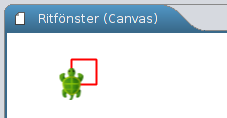
\includegraphics[width=0.47\textwidth]{../img/kojo/kvadrat}

\noindent Prova gärna olika sätt att skriva din kod \emph{utan} att resultatet ändras: skriv satser i sekvens på flera rader eller satser i sekvens på samma rad med semikolon emellan; använd blanktecken och blanka rader i koden. Hur vill du gruppera dina satser så att de är lätta för en människa att läsa?
%Prova att ändra på \emph{ordningen} mellan satserna och studera hur resultatet påverkas. Använd den \emph{gula} play-knappen  (programspårning) för att studera exekveringen i detalj. Vad händer du klickar på satser i ditt program och på rutor i programspårningen?


\Subtask Rita en trappa enligt bilden nedan.


\includegraphics[width=0.3\textwidth]{../img/kojo/stairs}

\Subtask Rita valfri bild på valfri bakgrund med hjälp av några av procedurerna i tabellen nedan. Du kan till exempel rita en rosa triangel med lila konturer mot svart bakgrund. % \ref{lab:kojo:kojo-procedures}. 
Försök att underlätta läsbarheten av din kod med hjälp av lämpliga radbrytningar och gruppering av satser. 


\begin{table}[H]
\begin{longtable}{l l}\small
\code|fram(100)| & Paddan går framåt 100 steg (25 om argument saknas).\\
\code|färg(rosa)| & Sätter pennans färg till rosa. \\
\code|fyll(lila)| & Sätter ifyllnadsfärgen till lila. \\
\code|fyll(genomskinlig)| & Gör så att paddan \emph{inte} fyller i något när den ritar. \\
\code|bredd(20)| & Gör så att pennan får bredden 20. \\
\code|bakgrund(svart)| & Bakgrundsfärgen blir svart. \\
\code|bakgrund2(grön,gul)| & Bakgrund med övergång från grönt till gult. \\
\code|pennaNer|  & Sätter ner paddans penna så att den ritar när den går. \\
\code|pennaUpp|  & Sänker paddans penna så att den \emph{inte} ritar när den går. \\
\code|höger(45)|   & Paddan vrider sig 45 grader åt höger. \\
\code|vänster(45)| & Paddan vrider sig 45 grader åt vänster. \\
\code|hoppa|       & Paddan hoppar 25 steg utan att rita. \\
\code|hoppa(100)|  & Paddan hoppar 100 steg utan att rita. \\
\code|hoppaTill(100, 200)| & Paddan hoppar till läget (100, 200) utan att rita. \\
\code|gåTill(100, 200)|    & Paddan vrider sig och går till läget (100, 200). \\
\code|öster|   & Paddan vrider sig så att nosen pekar åt höger. \\
\code|väster|  & Paddan vrider sig så att nosen pekar åt vänster. \\
\code|norr|    & Paddan vrider sig så att nosen pekar uppåt. \\
\code|söder|   & Paddan vrider sig så att nosen pekar neråt. \\
\code|mot(100,200)|   & Paddan vrider sig så att nosen pekar mot läget (100, 200) \\
\code|sättVinkel(90)| & Paddan vrider nosen till vinkeln 90 grader. \\
\end{longtable}
%\label{lab:kojo:kojo-procedures}
%\caption{Några användbara procedurer i Kojo.}
\end{table}

\begin{framed}
\noindent\emph{Tips inför fortsättningen:} Ha gärna både REPL och Kojo igång samtidigt. Då kan du undersöka hur olika kodkonstruktioner fungerar i REPL, medan du stegvis skapar allt större program i editorn i Kojo. Detta sätt att jobba har du nytta av under resten av kursen, både om du använder en texteditor och kompilerar i terminalen, och om du använder en professionell integrerad utvecklingsmiljö. Oavsett vilka andra verktyg du kör är det användbart att ha REPL igång i ett eget fönster som hjälp i den kreativa processen, medan du jagar buggar och medan du lär dig nya koncept. Så fort du undrar hur något fungerar i Scala: fram med REPL och testa!
\end{framed}


\SOLUTION

\TaskSolved \what
 
\SubtaskSolved Genom att börja din Kojo-program med \code{sudda} så startar du exekveringen i samma utgångsläge: en tom rityta \Eng{canvas} där paddan pekar uppåt, pennan är nere och pennans färg är röd.  Då blir det lättare att resonera om vad programmet gör från början till slut, jämfört med om exekveringen beror på resultatet av tidigare exekveringar.


\SubtaskSolved
\begin{Code}
sudda

fram; vänster
fram; vänster
fram; vänster
fram; vänster
\end{Code}


\SubtaskSolved
\begin{Code}
sudda

fram; vänster
fram; höger

fram; vänster
fram; höger

fram; vänster
fram; höger

fram; vänster
\end{Code}


\QUESTEND









\clearpage

\ExtraTasks %%%%%%%%%%%%%%%%%% EXTRAUPPGIFTER



\def\what{\emph{Typ och värde.}}

\QUESTBEGIN

\Task \what~Vilket värde och vilken typ hör till vilket uttryck?  Är du osäker på svaret, testa i REPL.

\begin{ConceptConnections}[0.3\textwidth]
  \code|1.0 + 18          | & 1 & & A & \code|42.0: Double    | \\ 
  \code|(41 + 1).toDouble | & 2 & & B & \code|65: Int         | \\ 
  \code|1.042e42 + 1      | & 3 & & C & \code|19.0: Double    | \\ 
  \code|12E6.toLong       | & 4 & & D & \code|12000000: Long  | \\ 
  \code|32.toChar.toString| & 5 & & E & \code|'*': Char       | \\ 
  \code|'A'.toInt         | & 6 & & F & \code|48: Int         | \\ 
  \code|0.toInt           | & 7 & & G & \code|" ": String   | \\ 
  \code|'0'.toInt         | & 8 & & H & \code|1.042E42: Double| \\ 
  \code|'9'.toInt         | & 9 & & I & \code|'q': Char       | \\ 
  \code|'A' + '0'         | & 10 & & J & \code|113: Int        | \\ 
  \code|('A' + '0').toChar| & 11 & & K & \code|0: Int          | \\ 
  \code|"*!%#".charAt(0)| & 12 & & L & \code|57: Int         | \\ 
\end{ConceptConnections}

\SOLUTION

\TaskSolved \what

\begin{ConceptConnections}
  \code|1.0 + 18          | & 1 & ~~\Large$\leadsto$~~ &  E & \code|19.0: Double    | \\ 
  \code|(41 + 1).toDouble | & 2 & ~~\Large$\leadsto$~~ &  L & \code|42.0: Double    | \\ 
  \code|1.042e42 + 1      | & 3 & ~~\Large$\leadsto$~~ &  A & \code|1.042E42: Double| \\ 
  \code|12E6.toLong       | & 4 & ~~\Large$\leadsto$~~ &  K & \code|12000000: Long  | \\ 
  \code|32.toChar.toString| & 5 & ~~\Large$\leadsto$~~ &  G & \code|" ": String   | \\ 
  \code|'A'.toInt         | & 6 & ~~\Large$\leadsto$~~ &  H & \code|65: Int         | \\ 
  \code|0.toInt           | & 7 & ~~\Large$\leadsto$~~ &  I & \code|0: Int          | \\ 
  \code|'0'.toInt         | & 8 & ~~\Large$\leadsto$~~ &  F & \code|48: Int         | \\ 
  \code|'9'.toInt         | & 9 & ~~\Large$\leadsto$~~ &  D & \code|57: Int         | \\ 
  \code|'A' + '0'         | & 10 & ~~\Large$\leadsto$~~ &  B & \code|113: Int        | \\ 
  \code|('A' + '0').toChar| & 11 & ~~\Large$\leadsto$~~ &  J & \code|'q': Char       | \\ 
  \code|"*!%#".charAt(0)| & 12 & ~~\Large$\leadsto$~~ &  C & \code|'*': Char       | \\ 
\end{ConceptConnections}

%\Subtask \code{1.0 + 18}
%
%\Subtask \code{(41 + 1).toDouble}
%
%\Subtask \code{1.042e42 + 1}
%
%\Subtask \code{12E6.toLong}
%
%\Subtask \code{"gurk" + 'a'}
%
%\Subtask \code{32.toChar.toString}
%
%\Subtask \code{'A'.toInt}
%
%\Subtask \linebreak[0] \code{'0'.toInt}
%
%\Subtask \code{'0'.toInt}
%
%\Subtask \code{'9'.toInt}
%
%\Subtask \code{'A' + '0'}
%
%\Subtask \code{('A' + '0').toChar}
%
%\Subtask \code{"*!%#".charAt(0)}
%%%%%%%%%%%%%%%%%%%%%%%%%%%%%%%%%%%%%%%%%%%%%%%%
%\SubtaskSolved \code{Double, 19}
%
%\SubtaskSolved \code{Double, 42}
%
%\SubtaskSolved \code{Double, 1.042E42}
%
%\SubtaskSolved \code{Long, 12000000}
%
%\SubtaskSolved \code{String, gurka}
%
%\SubtaskSolved \code{String, " "}
%
%\SubtaskSolved \code{Int, 65}
%
%\SubtaskSolved \code{Int, 48}
%
%\SubtaskSolved \code{Int,49}
%
%\SubtaskSolved \code{Int,57}
%
%\SubtaskSolved \code{Int, 113}
%
%\SubtaskSolved \code{Char, 'q'}
%
%\SubtaskSolved \code{Char, '*'}


\QUESTEND




\def\what{\emph{Satser och uttryck.}}

\QUESTBEGIN

\Task \what

\Subtask Vad är det för skillnad på en sats och ett uttryck?

\Subtask Ge exempel på satser som inte är uttryck?

\Subtask Förklara vad som händer för varje evaluerad rad:
\begin{REPL}
scala> def värdeSaknas = ()
scala> värdeSaknas
scala> värdeSaknas.toString
scala> println(värdeSaknas)
scala> println(println("hej"))
\end{REPL}

\Subtask Vilken typ har literalen \code{()}?

\Subtask Vilken returtyp har \code{println}?

\SOLUTION

\TaskSolved \what

\SubtaskSolved  Ett utryck kan evalueras och resulterar då i ett användbart värde. En sats \emph{gör} något (t.ex. skriver ut något), men resulterat inte i något användbart värde.

\SubtaskSolved \code{println()}

\SubtaskSolved 

 Värdesaknas innehåller Unit

 Skriver ut \code{Unit}

 Skriver ut \code{"()"}

 Skriver ut \code{"()"}

 Skriver först ut hej med det innersta anropet och sen \code{()} med det yttre anropet

\SubtaskSolved  \code{Unit}

\SubtaskSolved  \code{Unit}

\QUESTEND



\def\what{\emph{Procedur med parameter.} \TODO}

\QUESTBEGIN

\Task \what~En procedur är en funktion som orsakar en effekt, till exempel en utskrift eller en variabeltilldelning, men som inte returnerar något intressant resultatvärde. \footnote{I Scala är procedurer funktioner som returnerar det \emph{tomma värdet}, vilket skrivs \code{()} och är av typen \code{Unit}. I Java och flera andra språk finns inget tomt värde och man har en specialsyntax för procedurer som använder nyckelordet \code{void}. }

\Subtask Deklarera en förändringsbar variabel \code{highscore} som initieras till 0.

\Subtask Deklarera en procedur \code{updateHighscore} som tar en parameter \code{points} och tilldelar \code{highscore} \TODO ...


\SOLUTION

\TaskSolved \what

\SubtaskSolved 

\QUESTEND





\def\what{\emph{\code{if}\textit{-sats}.}}

\QUESTBEGIN

\Task \what~För varje rad nedan, beskriv vad som skrivs ut.  % Uppgift 18
\begin{REPL}
scala> if (!true) println("sant") else println("falskt")
scala> if (!false) println("sant") else println("falskt")
scala> def singlaSlant = if (math.random > 0.5) "krona" else "klave"
scala> for (i <- 1 to 5) print(s"$i:$singlaSlant ")
\end{REPL}

\SOLUTION

\TaskSolved \what

\begin{enumerate}
\item Utskrift: \code{falskt}
\item Utskrift: \code{sant}
\item Inget skrivs ut, funktionen deklareras men körs ej.
\item Utskrift: code{1:krona 2:klave 3:krona 4:krona 5:klave }
\end{enumerate}

\QUESTEND





\def\what{\emph{\code{if}\textit{-uttryck}.}}

\QUESTBEGIN

\Task  Deklarera följande variabler med nedan initialvärden:  

\begin{REPLnonum}
scala> var grönsak = "gurka"
scala> var frukt = "banan"
\end{REPLnonum}

Ange för varje rad nedan vad uttrycket har för värde och typ:
\begin{REPLnonum}
scala> if (grönsak == "tomat") "gott" else "inte gott" 
scala> if (frukt == "banan") "gott" else "inte gott" 
scala> if (true) grönsak else 42 
scala> if (false) grönsak else 42 
\end{REPLnonum}

\SOLUTION


\TaskSolved \what~Notera typen \code{Any} på de sista två uttrycken.

\begin{REPLnonum}
scala> if (grönsak == "tomat") "gott" else "inte gott"
res0: String = inte gott

scala> if (frukt == "banan") "gott" else "inte gott"
res1: String = gott

scala> if (true) grönsak else 42
res2: Any = gurka

scala> if (false) grönsak else 42
res3: Any = 42
\end{REPLnonum}


\QUESTEND






\def\what{\emph{QUESTTEMPLATE}}

\QUESTBEGIN

\Task \what

\Subtask

\SOLUTION

\TaskSolved \what

\SubtaskSolved 

\QUESTEND




\clearpage

\AdvancedTasks   %%%%%%%%%%%%%%%%%%% FÖRDJUPNINGSUPPGIFTER




\def\what{\emph{Stränginterpolatorn \code{s}.}}

\QUESTBEGIN

\Task \what~Med ett \code{s} framför en strängliteral får man hjälp av kompilatorn att, på ett typsäkert sätt, infoga variabelvärden i en sträng. 
Variablernas namn ska föregås med ett dollartecken, t.ex. \code{s"Hej $namn"}.  
Om man vill evaluera ett uttryck placeras detta inom klammer direkt efter dollartecknet, t.ex.
\code/s"Dubbla längden: ${namn.size * 2}"/  

\Subtask Vad skrivs ut nedan?
\begin{REPL}
scala> val f = "Kim"
scala> val e = "Finkodare"
scala> println(s"Namnet '$f $e' har ${f.size + e.size} bokstäver.")
\end{REPL}

\Subtask Skapa följande utskrifter med hjälp av stränginterpolatorn \code{s} och variablerna \code{f} och \code{e} i föregående deluppgift.
\begin{REPL}
Kim har 3 bokstäver.
Finkodare har 9 bokstäver.
\end{REPL}

\SOLUTION

\TaskSolved \what

\SubtaskSolved 
\begin{REPLnonum}
Namnet 'Kim Finkodare' har 12 bokstäver.
\end{REPLnonum}

\SubtaskSolved 
\begin{REPLnonum}
println(s"$f har  ${f.size} bokstäver.")
println(s"$e har  ${e.size} bokstäver.")
\end{REPLnonum}

\QUESTEND






\def\what{\emph{Flyttalsaritmetik}}

\QUESTBEGIN

\Task \what

\Subtask Vilket är det minsta positiva värdet av typen \code{Double}?

\Subtask Vad är värdet av detta uttryck? Varför blir det så?
\begin{REPL}
scala> Double.MaxValue + Double.MinPositiveValue == Double.MaxValue
\end{REPL}

\SOLUTION

\TaskSolved \what

\SubtaskSolved 

\begin{REPL}
scala> Double.MinPositiveValue
res0: Double = 4.9E-324
\end{REPL}

\SubtaskSolved 

\begin{REPL}
scala> Double.MaxValue + Double.MinPositiveValue == Double.MaxValue
res2: Boolean = true
\end{REPL}

\QUESTEND




\def\what{\emph{Stora tal.}}

\QUESTBEGIN

\Task \what~Om vi vill beräkna $2^{64} -1$ som ett exakt heltal\footnote{\url{https://en.wikipedia.org/wiki/Wheat_and_chessboard_problem}} blir det större än \code{Int.MaxValue}, så vi kan tyvärr inte använda snabba \code{Int}. Till vår räddning: \code{BigInt} 

\Subtask Läs om \code{BigInt} och \code{BigDecimal} på \Scaladoc \\ Notera vad de kan användas till. 

\Subtask Du skapar ett \code{BigInt}-heltal med \code{BigInt(2)} och kan anropa funktionen \code{pow} på en \code{BigInt} med punktnotation. Beräkna $2^{64} -1$ som ett exakt heltal.

\Subtask Vilka nackdelar finns med \code{BigInt} och \code{BigDecimal}?

\SOLUTION

\TaskSolved \what

\SubtaskSolved \code{BigInt} kan användas i stället för \code{Int} vid mycket stora heltal. \code{BigDecimal} kan användas i stället för \code{Double} vid mycket stora decimaltal.

\SubtaskSolved 
\begin{REPL}
scala> BigInt(2).pow(64)
res0: scala.math.BigInt = 18446744073709551616
\end{REPL}

\SubtaskSolved Beräkningar går mycket långsammare och de är lite krångligare att använda.

\QUESTEND





\def\what{\emph{Precedensregler}}

\QUESTBEGIN

\Task \what~Evalueringsordningen kan styras med parenteser. Vilket värde och vilken typ har följande uttryck? 

\Subtask \code{23 + 2 * 2 + (23 + 2) * 2}

\Subtask \code{(-(2 - 42)) / (1 + 1 + 1)}

\Subtask \code{(-(2 - 42)) / (-1)/(1 + 1 + 1)}

\SOLUTION

\TaskSolved \what

\SubtaskSolved \code{77:  Int}

\SubtaskSolved \code{13: Int}

\SubtaskSolved \code{-13: Int}

\QUESTEND






\def\what{\emph{QUESTTEMPLATE}}

\QUESTBEGIN

\Task \what

\Subtask

\SOLUTION

\TaskSolved \what

\SubtaskSolved 

\QUESTEND




\subsection{TODO}

\TODO{SAKERNA NEDAN SKA FLYTTAS/UPPDATERAS/TAS BORT???} 
%%%%%%%%%%%%%%%%%%%%%%%%%%%%%%%%%%%%%%%%%%%%%%%%
%%%%%%%%%%%%%%%%%%%%%%%%%%%%%%%%%%%%%%%%%%%%%%%%
%%%%%%%%%%%%%%%%%%%%%%%%%%%%%%%%%%%%%%%%%%%%%%%%
%%%%%%%%%%%%%%%%%%%%%%%%%%%%%%%%%%%%%%%%%%%%%%%%
%%%%%%%%%%%%%%%%%%%%%%%%%%%%%%%%%%%%%%%%%%%%%%%%
%%%%%%%%%%%%%%%%%%%%%%%%%%%%%%%%%%%%%%%%%%%%%%%%
%%%%%%%%%%%%%%%%%%%%%%%%%%%%%%%%%%%%%%%%%%%%%%%%
%%%%%%%%%%%%%%%%%%%%%%%%%%%%%%%%%%%%%%%%%%%%%%%%
%%%%%%%%%%%%%%%%%%%%%%%%%%%%%%%%%%%%%%%%%%%%%%%%


\ifPreSolution  %%% TODO remove \fi at end of file and break sultions into pieces





\Task Klassen \code{java.lang.Math} och paketobjektet \code{scala.math}. % Uppgift 11
Genom att trycka på tab tagenten kan man se vad som finns i olika paket.

\begin{REPL}
scala> java.    //tryck TAB efter punkten
applet   awt   beans   io   lang   math   net   nio   rmi   security   sql

scala>
\end{REPL}

\Subtask Undersök genom att trycka på Tab-tangenten, vilka funktioner som finns i \code{Math} och \code{math}. Vad heter konstanten $\pi$ i java.lang.Math respektive scala.math?

\begin{REPL}
scala> java.lang.Math.    //tryck TAB efter punkten
scala> scala.math.        //tryck TAB efter punkten
\end{REPL}

\Subtask Undersök dokumentationen för klassen \code{java.lang.Math} här: \\ \url{https://docs.oracle.com/javase/8/docs/api/java/lang/Math.html} \\
Vad gör \code{java.lang.Math.hypot}?

\Subtask Undersök dokumentationen för paketobjektet \code{scala.math} här: \\
\url{http://www.scala-lang.org/api/current/#scala.math.package} \\
Ge exempel på någon funktion i \code{java.lang.Math} som inte finns i \code{scala.math}.

%\TaskSection{Noggrannhet och undantag i aritmetiska uttryck}

\Task Vad händer här? Notera undantag \Eng{exceptions} och noggrannhetsproblem. % Uppgift 12

\Subtask \code{Int.MaxValue} + 1

\Subtask \code{1 / 0}

\Subtask \code{1E8 + 1E-8}

\Subtask \code{1E9 + 1E-9}

\Subtask \code{math.pow(math.hypot(3,6), 2)}

\Subtask \code{1.0 / 0}

\Subtask \code{(1.0 / 0).toInt}

\Subtask \code{math.sqrt(-1)}

\Subtask \code{math.sqrt(Double.NaN)}

\Subtask \code{throw new Exception("PANG!!!")}





\Task \textit{Deklarationer: \code{var}, \code{val}, \code{def}}. Evaluera varje rad nedan i tur och ordning i Scala REPL.  % Uppgift 15
\begin{REPL}[numbers=left, numberstyle=\color{black}\ttfamily\scriptsize\selectfont]
scala> var x = 30
scala> x + 1
scala> x
scala> x = x + 1
scala> x
scala> x == x + 1
scala> val y = 20
scala> y = y + 1
scala> var z = {println("gurka"); 10}
scala> def w = {println("gurka"); 10}
scala> z
scala> z
scala> z = z + 1
scala> w
scala> w
scala> w = w + 1
\end{REPL}

\Subtask För varje rad ovan: förklara för vad som händer.

\Subtask Vilka rader ger kompileringsfel och i så fall vilket och varför?

\Subtask\Pen Vad är det för skillnad på \code{var}, \code{val} och \code{def}?

\Subtask\Pen Tilldela variabeln \code{val even } värdet av ett uttryck som med modulo-operatorn \code
och olikhetsoperatorn \code{!=} testar om ett tal \code{n} är udda.


\Task\Pen \emph{Tilldelningsoperatorer.} Man kan förkorta en tilldelningssats som förändrar en variabel, t.ex. \code{x = x + 1}, genom att använda så kallade tilldelningsoperatorer och skriva \code{x += 1} som betyder samma sak. Rita en ny bild av datorns minne efter varje evaluerad rad nedan. Bilderna ska visa variablers namn, typ och värde.  % Uppgift 16

\begin{REPL}
scala> var a = 40
scala> var b = a + 40
scala> a += 10
scala> b -= 10
scala> a *= 2
scala> b /= 2
\end{REPL}



\Task \emph{Stränginterpolatorn \code{s}.} Man behöver ofta skapa strängar som innehåller variabelvärden. Med ett \code{s} framför en strängliteral får man hjälp av kompilatorn att, på ett typsäkert sätt, infoga variabelvärden i en sträng. Variablernas namn ska föregås med ett dollartecken, t.ex. \code{s"Hej $namn"}.  Om man vill evaluera ett uttryck placeras detta inom klammer direkt efter dollartecknet, t.ex.
\code/s"Dubbla längden: ${namn.size * 2}"/  % Uppgift 17

\begin{REPL}
scala> val f = "Kim"
scala> val e = "Finkodare"
scala> val tot = f.size + e.size
scala> println(s"Namnet '$f $e' har $tot bokstäver.")
scala> println(s"Efternamnet '$e' har ${e.size} bokstäver.")
\end{REPL}

\Subtask Vad skrivs ut ovan?

\Subtask Skapa följande utskrifter med hjälp av stränginterpolatorn \code{s} och lämpliga variabler.
\begin{REPL}
Namnet 'Kim' har 3 bokstäver.
Namnet 'Finkodare' har 9 bokstäver.
\end{REPL}



\Task \code{if}\textit{-sats}.För varje rad nedan; förklara vad som händer.  % Uppgift 18
\begin{REPL}
scala> if (true) println("sant") else println("falskt")
scala> if (false) println("sant") else println("falskt")
scala> if (!true) println("sant") else println("falskt")
scala> if (!false) println("sant") else println("falskt")
scala> def singlaSlant =
scala> 	 if (math.random > 0.5) print(" krona") else print(" klave")
scala> singlaSlant; singlaSlant; singlaSlant
\end{REPL}


\Task \code{if}\textit{-uttryck}. Deklarera följande variabler med nedan initialvärden:  % Uppgift 19

\begin{REPLnonum}
scala> var grönsak = "gurka"
scala> var frukt = "banan"
\end{REPLnonum}

Vad har följande uttryck för värden och typ?

\Subtask \code{if (grönsak == "tomat") "gott" else "inte gott" }

\Subtask \code{if (frukt == "banan") "gott" else "inte gott" }

\Subtask \code{if (frukt.size == grönsak.size) "lika stora" else "olika stora" }

\Subtask \code{if (true) grönsak else frukt }

\Subtask \code{if (false) grönsak else frukt }


\Task \code{for}\textit{-sats}.  Med bakåtpilen \texttt{<-} kan man i en \code{for}-sats ange vilka värden som ska gås igenom i sekvens. Vid varje runda i loopen får en lokal variabel ett nytt värde i sekvensen. % Uppgift 20

\Subtask Vad ger nedan \code{for}-satser för utskrift?

\begin{REPL}
scala> for (i <- 1 to 10) print(i + ", ")
scala> for (i <- 1 until 10) print(i + ", ")
scala> for (i <- 1 to 5) print((i * 2) + ", ")
scala> for (i <- 1 to 92 by 10) print(i + ", ")
scala> for (i <- 10 to 1 by -1) print(i + ", ")
\end{REPL}

\Subtask Skriv en \code{for}-sats som ger följande utskrift:
\begin{REPLnonum}
A1, A4, A7, A10, A13, A16, A19, A22, A25, A28, A31, A34, A37, A40, A43,
\end{REPLnonum}

\Task Repetition med metoden \code{foreach}. Efter framåtpilen \texttt{=>} (se nedan) anges vad som ska hända för varje element som gås igenom sekventiellt. Vid varje runda i loopen får en lokal variabel ett nytt värde i sekvensen.   % Uppgift 21

\Subtask Vad ger nedan satser för utskrifter?

\begin{REPL}
scala> (9 to 19).foreach{i => print(i + ", ")}
scala> (1 until 20).foreach{i => print(i + ", ")}
scala> (0 to 33 by 3).foreach{i => print(i + ", ")}
\end{REPL}

\Subtask Använd \code{foreach} och skriv ut följande:
\begin{REPLnonum}
B33, B30, B27, B24, B21, B18, B15, B12, B9, B6, B3, B0,
\end{REPLnonum}

\Task \code{while}\textit{-sats}. En sats eller ett block med satser upprepas så länge ett villkor är sant.  % Uppgift 22

\Subtask Vad ger nedan satser för utskrifter?
\begin{REPL}
scala> var i = 0
scala> while (i < 10) { println(i); i = i + 1 }
scala> var j = 0; while (j <= 10) { println(j); j = j + 2 }; println(j)
\end{REPL}

\Subtask Skriv en \code{while}-sats som ger följande utskrift. Använd en variabel \code{k} som initialiseras till 1.
\begin{REPLnonum}
A1, A4, A7, A10, A13, A16, A19, A22, A25, A28, A31, A34, A37, A40, A43,
\end{REPLnonum}

\Subtask\Pen Vilken av \code{for}, \code{while} och \code{foreach} är kortast att skriva om man vill repetera mer än en sats 100 gånger? Vilken tycker du är lättast att läsa?

\Task \textit{Slumptal}. Undersök vad dokumentationen säger om funktionen \code{scala.math.random}:\\  % Uppgift 23
\url{http://www.scala-lang.org/api/current/#scala.math.package}

\Subtask\Pen Vilken typ har värdet som returneras av funktionen \code{random}?

\Subtask\Pen Vilket är det minsta respektive största värde som kan returneras?

\Subtask\Pen Är \code{random} en \textit{äkta} funktion \Eng{pure function} i matematisk mening?

\Subtask Anropa funktionen \code{math.random} upprepade gånger och notera vad som händer. Använd pil-upp-tangenten.
\begin{REPLnonum}
scala> math.random
\end{REPLnonum}


\Subtask Vad händer? Använd \textit{pil-upp} och kör nedan \code{for}-sats flera gånger. Förklara vad som sker.

\begin{REPLnonum}
scala> for (i <- 1 to 20) println((math.random * 3 + 1).toInt)
\end{REPLnonum}

\Subtask Skriv en \code{for}-sats som skriver ut 100 slumpmässiga heltal från 0 till och med 9 på var sin rad.

\begin{REPLnonum}
scala> for (i <- 1 to 100) println(???)
\end{REPLnonum}

\Subtask Skriv en \code{for}-sats som skriver ut 100 slumpmässiga heltal från 1 till och med 6 på samma rad.

\begin{REPLnonum}
scala> for (i <- 1 to 100) print(???)
\end{REPLnonum}


\Subtask Använd \textit{pil-upp} och kör nedan \code{while}-sats flera gånger. Förklara vad som sker.

\begin{REPLnonum}
scala> while (math.random > 0.2) println("gurka")
\end{REPLnonum}

\Subtask Ändra i \code{while}-satsen ovan så att sannolikheten ökar att riktigt många strängar ska skrivas ut.

\Subtask Förklara vad som händer nedan.
\begin{REPL}
scala> var slumptal = math.random
scala> while (slumptal > 0.2) { println(slumptal); slumptal = math.random }
\end{REPL}

\Task\Pen \textit{Logik och De Morgans Lagar}. Förenkla följande uttryck. Antag att \code{poäng} och \code{highscore} är heltalsvariabler medan \code{klar} är av typen \code{Boolean}.
  % Uppgift 24

\Subtask \code{poäng > 100 && poäng > 1000}

\Subtask \code{poäng > 100 || poäng > 1000}

\Subtask \code{!(poäng > highscore)}

\Subtask \code{!(poäng > 0 && poäng < highscore) }

\Subtask \code{!(poäng < 0 || poäng > highscore) }

\Subtask \code{klar == true}

\Subtask \code{klar == false}


\clearpage

\ExtraTasks

\Task \textit{Slumptal}.

\Subtask Ersätt \code{???} nedan med literaler så att \code{tärning} returnerar ett slumpmässigt heltal mellan 1 och 6.
\begin{REPLnonum}
scala> def tärning = (math.random * ??? + ???).toInt
\end{REPLnonum}

\Subtask Ersätt \code{???} med literaler så att \code{rnd} blir ett decimaltal med max en decimal mellan 0.0 och 1.0.
\begin{REPLnonum}
scala> def rnd = math.round(math.random * ???) / ???
\end{REPLnonum}

\Subtask Vad blir det för skillnad om \code{math.round} ersätts med \code{math.floor} ovan? (Se dokumentationen av \code{java.lang.Math.round} och \code{java.lang.Math.floor}.)

\Task Undersök vad som finns i paketet \code{scala.math} genom att studera dess dokumentation: \href{http://www.scala-lang.org/api/current/#scala.math.package}{www.scala-lang.org/api/current/\#scala.math.package} och gör några matematiska beräkningar i REPL som använder olika funktioner i \code{math}-paketet.

\Task\Pen Antag att du byter plats mellan satsen efter villkoret och satsen efter \code{else} i \code{if}-satsen nedan. Hur kan du ändra i villkoret så att det ändå skrivs ut samma sak som före bytet?
\begin{Code}
if (x == 42) println("the meaning of it all") else println(":(")
\end{Code}

\Task\Pen Rita en ny bild av datorns minne efter varje evaluerad rad nedan. Bilderna ska visa variablers namn, typ och värde.
\begin{REPL}
scala> var x = 42
scala> var y = x + 1
scala> x += -1
scala> y -= 1
\end{REPL}

\Task Skapa med hjälp av \code{while} några olika oändliga loopar som skriver ut olika saker vid varje loop-runda.

\Task Hitta på några egna övningar för att träna mer på De Morgans lagar.



\clearpage

\AdvancedTasks

\Task Läs om moduloräkning här \href{https://en.wikipedia.org/wiki/Modulo\_operation}{en.wikipedia.org/wiki/Modulo\_operation} och undersök hur det blir med olika tecken (positivt resp. negativt) på divisor och dividend.



\Task Läs om identifierare i Scala och speciellt \emph{literal identifiers} här: \url{http://www.artima.com/pins1ed/functional-objects.html#6.10}.

\Subtask Förklara vad som händer nedan:
\begin{REPLnonum}
scala> val `konstig val` = 42
scala> println(`konstig val`)
\end{REPLnonum}

\Subtask Scala och Java har olika uppsättningar med reserverade ord. På vilket sätt kan ''backticks'' vara använbart med anledning av detta?


\Task Sök upp dokumentationen för \code{java.lang.Integer}.

\Subtask Undersök i REPL hur metoderna \code{toBinaryString} och \code{toHexString} fungerar.

\Subtask Vad betyder literalen \code{0x2a}?

\Task Typannoteringar skapas genom att i ett uttryck placera ett kolon följt av en typ, vid behov  omslutet av en parentes. Skapa ett större uttryck med typannoteringar och försök få kompilatorn att kontrollera typen på intressanta ställen. Märk att typannoteringar också ibland kan användas för att konvertera mellan numeriska typer.


\Task Förklara vad som händer nedan:
\begin{REPL}
scala> var i = 42
scala> i += 1
scala> i *= 2
scala> i /= 3
\end{REPL}


\Task Läs om BigInt och BigDecimal här: \href{http://alvinalexander.com/scala/how-to-use-large-integer-decimal-numbers-in-scala-bigint-bigdecimal}{alvinalexander.com/scala/how-to-use-large-integer-decimal-numbers-in-scala-bigint-bigdecimal} och prova att skapa riktigt stora tal med hjälp av metoden \code{pow} på BigInt och tal med riktigt många decimaler med BigDecimal dess metod \code{pow}.

\Task Sök upp dokumentationtionen för \code{java.lang.Math.multiplyExact} och läs om vad den metoden gör.

\Subtask Vad händer här?
\begin{REPLnonum}
scala> Math.multiplyExact(2, 42)
scala> Math.multiplyExact(Int.MaxValue, Int.MaxValue)
\end{REPLnonum}

\Subtask\Pen Varför kan man vilja använda \code{java.lang.Math.multiplyExact} i stället för ''vanlig'' multiplikation?



\Subtask\Pen Sök med Ctrl+F i webbläsaren och efter förekomster av texten \textit{''overflow''} i javadoc för klassen \code{java.lang.Math} i JDK 8. Vad är ''overflow''? Vilka metoder finns i \code{java.lang.Math} som hjälper dig att upptäcka om det blir overflow?

\Task Använda Scala REPL för att undersöka konstanterna nedan. Vilket av dessa värden är negativt? Vad kan man ha för praktisk nytta av dessa värden i ett program som gör flyttalsberäkningar?

\Subtask \code{java.lang.Double.MIN_VALUE}

\Subtask \code{scala.Double.MinValue}

\Subtask \code{scala.Double.MinPositiveValue}

\Task För typerna \code{Byte}, \code{Short}, \code{Char}, \code{Int}, \code{Long}, \code{Float}, \code{Double}: Undersök hur många bitar som behövs för att representera varje typs omfång? \\*
\textit{Tips:} Några användbara uttryck: \\*
 \code{Integer.toBinaryString(Int.MaxValue + 1).size} \\*
 \code{Integer.toBinaryString((math.pow(2,16) - 1).toInt).size} \\*
 \code{1 + math.log(Long.MaxValue)/math.log(2)}
Se även språkspecifikationen för Scala, kapitlet om heltalsliteraler: \\
\url{http://www.scala-lang.org/files/archive/spec/2.11/01-lexical-syntax.html#integer-literals}

\Subtask Undersök källkoden för paketobjektet \code{scala.math} här: \\
\url{https://github.com/scala/scala/blob/v2.11.7/src/library/scala/math/package.scala} \\
Hur många olika överlagrade varianter av funktionen \code{abs} finns det och för vilka parametertyper är den definierad?

\Task Läs mer om stränginterpolatorer här:\\ \href{http://docs.scala-lang.org/overviews/core/string-interpolation.html}{docs.scala-lang.org/overviews/core/string-interpolation.html} \\ Hur kan du använda \code{f}-interpolatorn för att göra följande utskrift i REPL? Byt ut \code{???} mot lämpliga tecken.
\begin{REPLnonum}
scala> val g: Double = 1 / 3.0
scala> val s: String = f"Gurkan är ??? meter lång"
scala> println(s)
Gurkan är 0.333 meter lång
\end{REPLnonum}

\fi %%% TODO fix solutions



